\documentclass[11pt,largemargins]{homework}

\newcommand{\hwname}{Shuyu Zhao}
\newcommand{\hwemail}{shuyu.zhao@connect.polyu.hk}
\newcommand{\hwtype}{Assignment}
\newcommand{\hwnum}{2}
\newcommand{\hwclass}{COMP5112}
\newcommand{\hwlecture}{}
\newcommand{\hwsection}{}

% This is just used to generate filler content. You don't need it in an actual
% homework!
\usepackage{lipsum}
\usepackage{tikz}
\usepackage{graphicx}
\usepackage{subfigure}
\usepackage[linesnumbered,boxed]{algorithm2e}
\usepackage{xifthen}
\usepackage{paratype}

\usetikzlibrary{matrix}
\usetikzlibrary{shapes,arrows,positioning,decorations,
  automata,backgrounds,petri,bending,
  shapes.multipart
} %Eventuell sind nicht alle nötig
\tikzset{
 array/.style = {rectangle split, rectangle split horizontal,
           draw}
}

\usepackage{pgf}

\usepackage{listings}
\usepackage{fontspec} % 定制字体
\newfontfamily\menlo{Menlo}
% \usepackage{xcolor} % 定制颜色
% \definecolor{mygreen}{rgb}{0,0.6,0}
% \definecolor{mygray}{rgb}{0.5,0.5,0.5}
% \definecolor{mymauve}{rgb}{0.58,0,0.82}
\lstset{ %
backgroundcolor=\color{white},      % choose the background color
basicstyle=\footnotesize\ttfamily,  % size of fonts used for the code
columns=fullflexible,
tabsize=4,
breaklines=true,               % automatic line breaking only at whitespace
captionpos=b,                  % sets the caption-position to bottom
escapeinside={\%*}{*)},        % if you want to add LaTeX within your code
keywordstyle=\color{blue},     % keyword style
frame=single,
rulesepcolor=\color{red!20!green!20!blue!20},
% identifierstyle=\color{red},
language=c++,
}

\begin{document}
\maketitle

\question
\begin{figure}[h!]
\centering
\subfigure[1.1]{
\begin{minipage}[c]{0.4\linewidth}
\centering
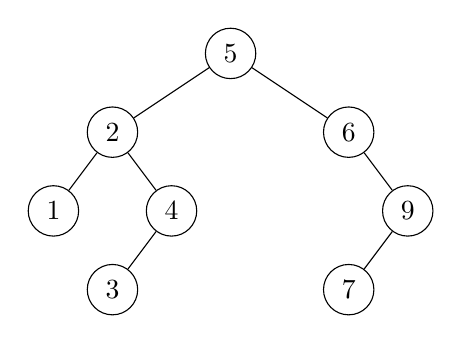
\begin{tikzpicture}[
    every node/.style={
        circle, draw,
        inner sep=0pt,
        text width=6mm,
        align=center
    },
    level distance=10mm,
    level 1/.style={sibling distance=30mm},
    level 2/.style={sibling distance=15mm}
]
\node{$5$}
child{node{$2$}  
    child{node{$1$}}
    child{node{$4$}
            child{node{$3$}}
            child[missing]} 
}
child{node{$6$}  
        child[missing]
        child{node{$9$} 
                child{node{$7$}}
                child[missing]}
};
\end{tikzpicture}
\end{minipage}
}
\subfigure[1.2]{
\begin{minipage}[c]{0.4\linewidth}
\centering
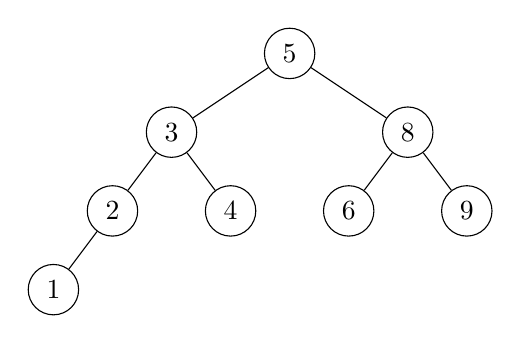
\begin{tikzpicture}[
    every node/.style={
        circle, draw,
        inner sep=0pt,
        text width=6mm,
        align=center
    },
    level distance=10mm,
    level 1/.style={sibling distance=30mm},
    level 2/.style={sibling distance=15mm}
]
\node{$5$}
child{node{$3$}  
    child{node{$2$} 
            child{node{$1$}}
            child[missing]}
    child{node{$4$}}
}
child{node{$8$}  
        child{node{$6$}}
        child{node{$9$}}
};
\end{tikzpicture}
\end{minipage}
}
\subfigure[1.3]{
\begin{minipage}[c]{0.4\linewidth}
\centering
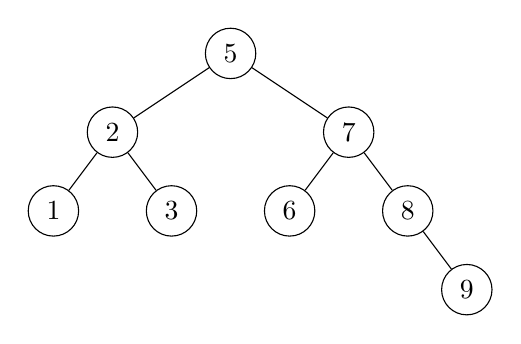
\begin{tikzpicture}[
    every node/.style={
        circle, draw,
        inner sep=0pt,
        text width=6mm,
        align=center
    },
    level distance=10mm,
    level 1/.style={sibling distance=30mm},
    level 2/.style={sibling distance=15mm}
]
\node{$5$}
child{node{$2$}  
    child{node{$1$}}
    child{node{$3$}}
}
child{node{$7$}  
        child{node{$6$}}
        child{node{$8$}
          child[missing]
          child{node{$9$}}}
};
\end{tikzpicture}
\end{minipage}
}

\caption{Problem 1}
\end{figure}

\question
  \begin{alphaparts}
    \questionpart A isn't a valid BST.(6 is small than 7 while 6 is on 7's right subtree)
    \questionpart B is a valid BST. Resultant Tree see Fig \ref{fig:21}.
    \questionpart C is a valid BST. Resultant Tree see Fig \ref{fig:22}.
    \questionpart D is a valid BST. Resultant Tree see Fig \ref{fig:23}.
    \questionpart E is a valid BST. Resultant Tree see Fig \ref{fig:24}.
  \end{alphaparts}

\begin{figure}[h!]
\centering
\subfigure[2.1]{
\label{fig:21}
\begin{minipage}[c]{0.3\linewidth}
\centering
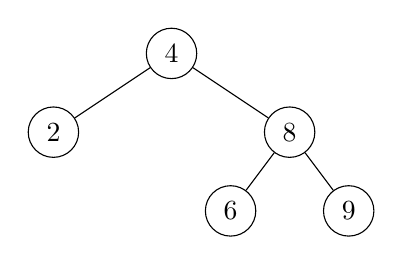
\begin{tikzpicture}[
    every node/.style={
        circle, draw,
        inner sep=0pt,
        text width=6mm,
        align=center
    },
    level distance=10mm,
    level 1/.style={sibling distance=30mm},
    level 2/.style={sibling distance=15mm}
]
\node{$4$}
child{node{$2$}}
child{node{$8$}  
        child{node{$6$}}
        child{node{$9$}}
};
\end{tikzpicture}
\end{minipage}
}
\subfigure[2.2]{
\label{fig:22}
\begin{minipage}[c]{0.3\linewidth}
\centering
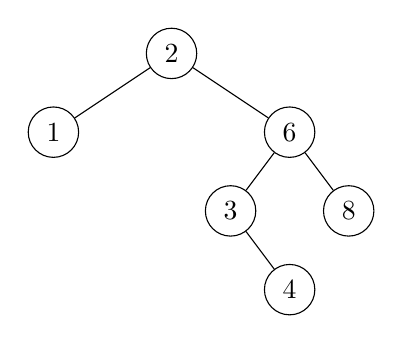
\begin{tikzpicture}[
    every node/.style={
        circle, draw,
        inner sep=0pt,
        text width=6mm,
        align=center
    },
    level distance=10mm,
    level 1/.style={sibling distance=30mm},
    level 2/.style={sibling distance=15mm}
]
\node{$2$}
child{node{$1$}}
child{node{$6$}  
        child{node{$3$}
          child[missing]
          child{node{$4$}}}
        child{node{$8$}}
};
\end{tikzpicture}
\end{minipage}
}
\subfigure[2.3]{
\label{fig:23}
\begin{minipage}[c]{0.3\linewidth}
\centering
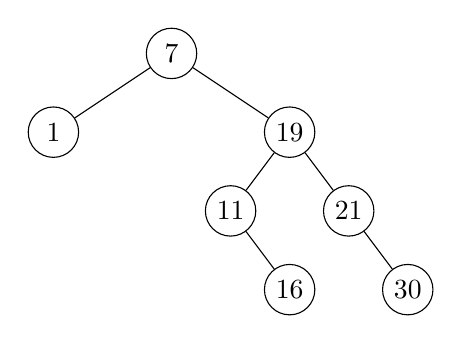
\begin{tikzpicture}[
    every node/.style={
        circle, draw,
        inner sep=0pt,
        text width=6mm,
        align=center
    },
    level distance=10mm,
    level 1/.style={sibling distance=30mm},
    level 2/.style={sibling distance=15mm}
]
\node{$7$}
child{node{$1$}}
child{node{$19$}  
        child{node{$11$}
          child[missing]
          child{node{$16$}}}
        child{node{$21$}
          child[missing]
          child{node{$30$}}}
};
\end{tikzpicture}
\end{minipage}
}

\subfigure[2.4]{
\label{fig:24}
\begin{minipage}[c]{0.3\linewidth}
\centering
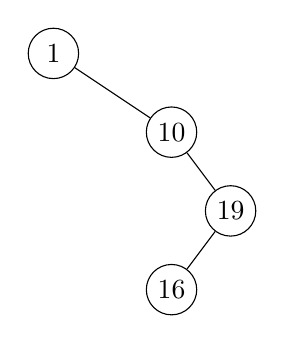
\begin{tikzpicture}[
    every node/.style={
        circle, draw,
        inner sep=0pt,
        text width=6mm,
        align=center
    },
    level distance=10mm,
    level 1/.style={sibling distance=30mm},
    level 2/.style={sibling distance=15mm}
]
\node{$1$}
child[missing]
child{node{$10$}  
        child[missing]
        child{node{$19$}
          child{node{$16$}}
          child[missing]}
};
\end{tikzpicture}
\end{minipage}
}
\caption{Problem 2}
\end{figure}

\question
Answer is \textbf{2}.

\question
My approach: put values in the binary tree to a list, then sort the list, do inorder traversel to the binary tree to put value into it finally. See pseudocode in Algorithm \ref{alg:1}.

The time complexity of this approach is decided by sorting algorithm. The minimum time complexity of this approach is $\mathcal{O}(nlogn)$ if we use quick sort. In general cases, the time complexity will be $\mathcal{O}(nlogn)$, however, the time complexity will be $\mathcal{O}(n^2)$ in the worst case(When the call tree of quick sort is the most unbalanced).

\begin{algorithm}
\label{alg:1}
\caption{Pseudocode for converting a binary tree to a BST}
\KwIn{$T$, A normal binary Tree}
\KwOut{$T$(in place editing)}
Create an empty list $L$\;
\SetKwFunction{FMain}{Store\_to\_list}
\SetKwProg{Fn}{Function}{:}{}
\Fn{\FMain{$T$, $L$}}{
    \If{$T=NULL$}{
      return\;
    }
    \FMain{$T.left$, $L$}\;
    append $T.data$ to $L$\;
    \FMain{$T.right$, $L$}\;
}

\SetKwFunction{Fp}{Partition}
\SetKwProg{Fn}{Function}{:}{}
\Fn{\Fp{$L$, $p$, $r$}}{
    $x=L[r]$\;
    $i=p-1$\;
    \For{$j=p$ to $j=r-1$}{
      \If{$L[j] \le x $}{
        $i=i+1$\;
        exchange $L[i]$ and $L[j]$\;
      }
    }
    exchange $L[i+1]$ and $L[r]$\;
    return $i+1$\;
}

\SetKwFunction{Fz}{Quick\_Sort}
\SetKwProg{Fn}{Function}{:}{}
\Fn{\Fz{$L$, $p$, $r$}}{
    \If{$p \textless r$}{
      $q$ = \Fp{$L$, $p$, $r$}\;
      \Fz{$L$, $p$, $q-1$}\;
      \Fz{$L$, $q+1$, $r$}\;
    }
}

Creat a temporary variable $flag=0$\;
\SetKwFunction{Fx}{Convert\_to\_BST}
\SetKwProg{Fn}{Function}{:}{}
\Fn{\Fx{$T$, $L$}}{
    \If{$T=NULL$}{
      return\;
    }
    \Fx{$T.left$, $L$}\;
    $T.data$=$L[flag]$\;
    $flag=flag+1$;

    \Fx{$T.right$, $L$}\;
}
\end{algorithm}

\question
If we choose one key as root, so it will have four situations:
\begin{enumerate}
  \item 0 key on left and 3 keys on right
  \item 3 keys on left and 0 key on left
  \item 1 key on left and 2 keys on right
  \item 2 keys on left and 1 key on right
\end{enumerate}

Hence, problem converts to how many different BST could created by 0/1/2/3 keys.

\begin{enumerate}
  \item With 0 key and 1 key, we can only create 1 type of BST.
  \item With 2 keys, we choose one key as root, so it will have 2 type of BST.
  \item With 3 keys, if we choose one key as root, so it will have three situations:
    \begin{enumerate}
      \item 0 key on left and 2 keys on right, result to 2 types
      \item 2 keys on left and 0 keys on right, result to 2 types
      \item 1 key on left and 1 key on right, result to 1 type
    \end{enumerate}
\end{enumerate}

So, we will have $2(2+2+1+2)=14$ types of BST with 4 keys in total. In general, we will have $C_{n}=\frac{(2n)!}{(n+1)!n!}$ types of BST with $n$ distinct keys.


\question
\begin{enumerate}
  \item \textbf{True}, in-order traversal always start from the left-most child(the smallest one) and end on the right-most child(the biggest one), which is an increasing order.
  \item \textbf{False}, we cannot reconstruct the BST based on one single traversal. Combinations of traversal(pre-order + in-order or post-order + in-order) can help us to construct the original BST. For instance, Using in-order traversal(1,2,3) and post-order(2,1,3) can construct one specific BST(1-2[root]-3), while we can construct three BSTs(1[root]-2-3, 1-2[root]-3, 1-2-3[root]) with only in-order traversal.
\end{enumerate}

\question
My approach: Do bottom-up comparison or upheap. See pseudocode in Algorithm \ref{alg:2}. The time complexity of this approach is $\mathcal{O}(n)$. Each time we call \textbf{Heapify}, it takes $\mathcal{O}(k)$, $k$ stands for the heap's height. Different nodes has different $k$ and we have $\frac{n}{2^(k+1)}$ nodes on height $k$. Hence, $T(n)=\left(\sum_{k=1}^{log(n)} \frac{1}{2^{k}} \times k\right){*} n$. Assume $S=\sum_{k=1}^{log(n)} \frac{1}{2^{k}} \times k$, $\frac{S}{2} = \sum_{k=1}^{log(n)-1} \frac{1}{2^{k}} \times k$, $S - \frac{S}{2} = \frac{S}{2} = \frac{1}{2}+\frac{1}{4}+\cdots+\frac{1}{2^{k}}-\frac{1}{2^{k+1}} \times k \leq 2$. So $T(n) \leq 2n = \mathcal{O}(n)$. Demo see Fig \ref{p7}.
\begin{algorithm}
\label{alg:2}
\caption{Pseudocode for converting an unsorted array to a Min heap}
\KwIn{$V$, An unsorted array, $i$, index of the array}
\KwOut{$V$, Min heap(in place editing)}
$l$ = Left[$i$]\;
$r$ = right[$i$]\;
\SetKwFunction{FMain}{Heapify}
\SetKwProg{Fn}{Function}{:}{}
\Fn{\FMain{$V$, $i$}}{
    \uIf{$l \le V$.heap-size and $V[l] \textless V[i]$}{
      $min = l$\;
    }
    \Else{
      $min = i$\;
    }
    \If{$r \le V$.heap-size and $V[r] \textless V[min]$}{
      $min = r$\;
    }
    \If{$min \neq i$}{
      exchange $V[i]$ and $V[min]$\;
      \FMain{$V$, $min$}
    }
}

$V$.heap-size = $V$.length\;
\For{$i = V.length \% 2$ to $1$}{
  \FMain{$V$, i}
}
\end{algorithm}

\begin{figure}[h!]
\centering
\subfigure[step 1]{
\begin{minipage}[c]{0.4\linewidth}
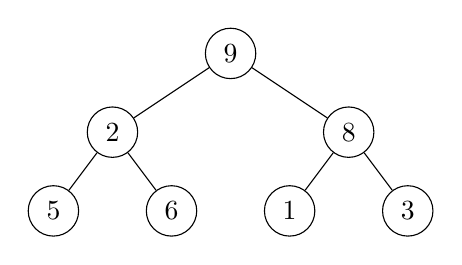
\begin{tikzpicture}[
    every node/.style={
        circle, draw,
        inner sep=0pt,
        text width=6mm,
        align=center
    },
    level distance=10mm,
    level 1/.style={sibling distance=30mm},
    level 2/.style={sibling distance=15mm}
]
\node{$9$}
child{node{$2$}
        child{node{$5$}}
        child{node{$6$}}}
child{node{$8$}  
        child{node{$1$}}
        child{node{$3$}}
};
\end{tikzpicture}
\end{minipage}
}
\subfigure[step 2]{
\begin{minipage}[c]{0.4\linewidth}
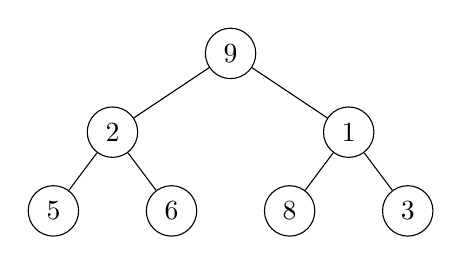
\begin{tikzpicture}[
    every node/.style={
        circle, draw,
        inner sep=0pt,
        text width=6mm,
        align=center
    },
    level distance=10mm,
    level 1/.style={sibling distance=30mm},
    level 2/.style={sibling distance=15mm}
]
\node{$9$}
child{node{$2$}
        child{node{$5$}}
        child{node{$6$}}}
child{node{$1$}  
        child{node{$8$}}
        child{node{$3$}}
};
\end{tikzpicture}
\end{minipage}
}
\subfigure[step 3]{
\begin{minipage}[c]{0.4\linewidth}
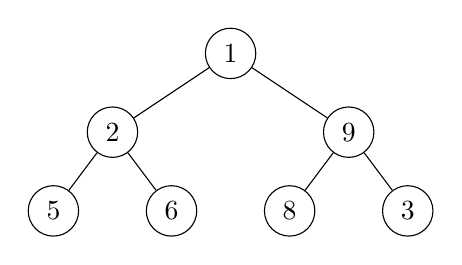
\begin{tikzpicture}[
    every node/.style={
        circle, draw,
        inner sep=0pt,
        text width=6mm,
        align=center
    },
    level distance=10mm,
    level 1/.style={sibling distance=30mm},
    level 2/.style={sibling distance=15mm}
]
\node{$1$}
child{node{$2$}
        child{node{$5$}}
        child{node{$6$}}}
child{node{$9$}  
        child{node{$8$}}
        child{node{$3$}}
};
\end{tikzpicture}
\end{minipage}
}
\subfigure[step 4]{
\begin{minipage}[c]{0.4\linewidth}
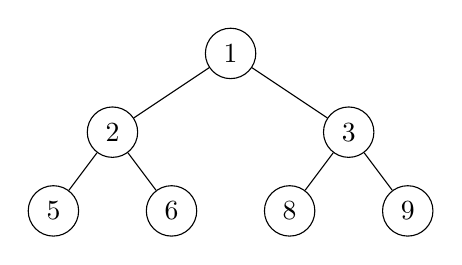
\begin{tikzpicture}[
    every node/.style={
        circle, draw,
        inner sep=0pt,
        text width=6mm,
        align=center
    },
    level distance=10mm,
    level 1/.style={sibling distance=30mm},
    level 2/.style={sibling distance=15mm}
]
\node{$1$}
child{node{$2$}
        child{node{$5$}}
        child{node{$6$}}}
child{node{$3$}  
        child{node{$8$}}
        child{node{$9$}}
};
\end{tikzpicture}
\end{minipage}
}
\caption{Problem 7}
\label{p7}
\end{figure}

\newpage
\question
The answer is \{null, 2, 4, 3, 9, 7, 6\}.

\question
The answer are \textbf{1},\textbf{3}.

\question
Answer see Fig \ref{hs10}, log see below.

\begin{figure}[h!]
\centering
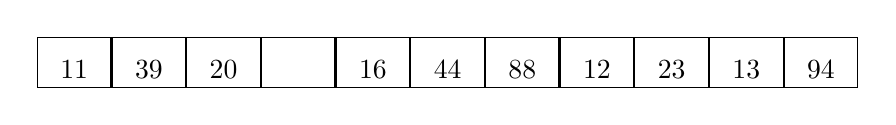
\begin{tikzpicture}
  \matrix[matrix of math nodes, nodes in empty cells, 
    nodes={draw,
    align=center,
    text width=0.7cm,
    text height=.4cm,
    minimum width=.7cm}
  ]{
    11 & 39 & 20 &  & 16 & 44 & 88 & 12 & 23 & 13 & 94\\
  };
% [11, 39, 20, 0, 16, 44, 88, 12, 23, 13, 94]
 \end{tikzpicture}
\caption{Problem 10}
\label{hs10}
\end{figure}

\begin{lstlisting}
12 Succ with hv = 7-[0, 0, 0, 0, 0, 0, 0, 12, 0, 0, 0]
44 Succ with hv = 5-[0, 0, 0, 0, 0, 44, 0, 12, 0, 0, 0]
13 Succ with hv = 9-[0, 0, 0, 0, 0, 44, 0, 12, 0, 13, 0]
88 Fail with hv = 5-[0, 0, 0, 0, 0, 44, 0, 12, 0, 13, 0]
88 Succ with hv = 6-[0, 0, 0, 0, 0, 44, 88, 12, 0, 13, 0]
23 Fail with hv = 7-[0, 0, 0, 0, 0, 44, 88, 12, 0, 13, 0]
23 Succ with hv = 8-[0, 0, 0, 0, 0, 44, 88, 12, 23, 13, 0]
94 Fail with hv = 6-[0, 0, 0, 0, 0, 44, 88, 12, 23, 13, 0]
94 Fail with hv = 7-[0, 0, 0, 0, 0, 44, 88, 12, 23, 13, 0]
94 Fail with hv = 8-[0, 0, 0, 0, 0, 44, 88, 12, 23, 13, 0]
94 Fail with hv = 9-[0, 0, 0, 0, 0, 44, 88, 12, 23, 13, 0]
94 Succ with hv = 10-[0, 0, 0, 0, 0, 44, 88, 12, 23, 13, 94]
11 Fail with hv = 5-[0, 0, 0, 0, 0, 44, 88, 12, 23, 13, 94]
11 Fail with hv = 6-[0, 0, 0, 0, 0, 44, 88, 12, 23, 13, 94]
11 Fail with hv = 7-[0, 0, 0, 0, 0, 44, 88, 12, 23, 13, 94]
11 Fail with hv = 8-[0, 0, 0, 0, 0, 44, 88, 12, 23, 13, 94]
11 Fail with hv = 9-[0, 0, 0, 0, 0, 44, 88, 12, 23, 13, 94]
11 Fail with hv = 10-[0, 0, 0, 0, 0, 44, 88, 12, 23, 13, 94]
11 Succ with hv = 0-[11, 0, 0, 0, 0, 44, 88, 12, 23, 13, 94]
39 Fail with hv = 6-[11, 0, 0, 0, 0, 44, 88, 12, 23, 13, 94]
39 Fail with hv = 7-[11, 0, 0, 0, 0, 44, 88, 12, 23, 13, 94]
39 Fail with hv = 8-[11, 0, 0, 0, 0, 44, 88, 12, 23, 13, 94]
39 Fail with hv = 9-[11, 0, 0, 0, 0, 44, 88, 12, 23, 13, 94]
39 Fail with hv = 10-[11, 0, 0, 0, 0, 44, 88, 12, 23, 13, 94]
39 Fail with hv = 0-[11, 0, 0, 0, 0, 44, 88, 12, 23, 13, 94]
39 Succ with hv = 1-[11, 39, 0, 0, 0, 44, 88, 12, 23, 13, 94]
20 Fail with hv = 1-[11, 39, 0, 0, 0, 44, 88, 12, 23, 13, 94]
20 Succ with hv = 2-[11, 39, 20, 0, 0, 44, 88, 12, 23, 13, 94]
16 Succ with hv = 4-[11, 39, 20, 0, 16, 44, 88, 12, 23, 13, 94]
\end{lstlisting}


\question
\begin{figure}[h!]

\centering
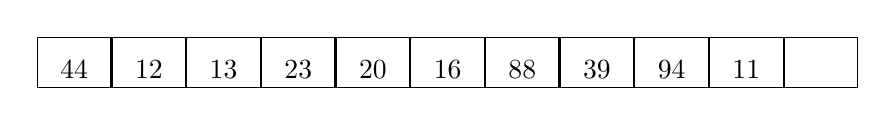
\begin{tikzpicture}
  \matrix[matrix of math nodes, nodes in empty cells, 
    nodes={draw,
    align=center,
    text width=0.7cm,
    text height=.4cm,
    minimum width=.7cm}
  ]{
    44 & 12 & 13 & 23 & 20 & 16 & 88 & 39 & 94 & 11 & \\
  };
% [44, 12, 13, 23, 20, 16, 88, 39, 94, 11, 0]
\end{tikzpicture}
\caption{Problem 11}
\label{hs11}
\end{figure}
Answer see Fig \ref{hs11}, log see below.

\begin{lstlisting}
12 Succ with i = 0, hv = 1-[0, 12, 0, 0, 0, 0, 0, 0, 0, 0, 0]
44 Succ with i = 0, hv = 0-[44, 12, 0, 0, 0, 0, 0, 0, 0, 0, 0]
13 Succ with i = 0, hv = 2-[44, 12, 13, 0, 0, 0, 0, 0, 0, 0, 0]
88 Fail with i = 0, hv = 0-[44, 12, 13, 0, 0, 0, 0, 0, 0, 0, 0]
88 Fail with i = 1, hv = 2-[44, 12, 13, 0, 0, 0, 0, 0, 0, 0, 0]
88 Succ with i = 0, hv = 6-[44, 12, 13, 0, 0, 0, 88, 0, 0, 0, 0]
23 Fail with i = 0, hv = 1-[44, 12, 13, 0, 0, 0, 88, 0, 0, 0, 0]
23 Succ with i = 0, hv = 3-[44, 12, 13, 23, 0, 0, 88, 0, 0, 0, 0]
94 Fail with i = 0, hv = 6-[44, 12, 13, 23, 0, 0, 88, 0, 0, 0, 0]
94 Succ with i = 0, hv = 8-[44, 12, 13, 23, 0, 0, 88, 0, 94, 0, 0]
11 Fail with i = 0, hv = 0-[44, 12, 13, 23, 0, 0, 88, 0, 94, 0, 0]
11 Fail with i = 1, hv = 2-[44, 12, 13, 23, 0, 0, 88, 0, 94, 0, 0]
11 Fail with i = 2, hv = 6-[44, 12, 13, 23, 0, 0, 88, 0, 94, 0, 0]
11 Fail with i = 3, hv = 1-[44, 12, 13, 23, 0, 0, 88, 0, 94, 0, 0]
11 Succ with i = 0, hv = 9-[44, 12, 13, 23, 0, 0, 88, 0, 94, 11, 0]
39 Fail with i = 0, hv = 6-[44, 12, 13, 23, 0, 0, 88, 0, 94, 11, 0]
39 Fail with i = 1, hv = 8-[44, 12, 13, 23, 0, 0, 88, 0, 94, 11, 0]
39 Fail with i = 2, hv = 1-[44, 12, 13, 23, 0, 0, 88, 0, 94, 11, 0]
39 Succ with i = 0, hv = 7-[44, 12, 13, 23, 0, 0, 88, 39, 94, 11, 0]
20 Fail with i = 0, hv = 9-[44, 12, 13, 23, 0, 0, 88, 39, 94, 11, 0]
20 Fail with i = 1, hv = 0-[44, 12, 13, 23, 0, 0, 88, 39, 94, 11, 0]
20 Succ with i = 0, hv = 4-[44, 12, 13, 23, 20, 0, 88, 39, 94, 11, 0]
16 Succ with i = 0, hv = 5-[44, 12, 13, 23, 20, 16, 88, 39, 94, 11, 0]
\end{lstlisting}


\question
\begin{enumerate}
  \item chaining: \textbf{pros}: It's easy to deal with collision with just adding value on the front or tail of the linked list. \textbf{cons}: It has to maintain many linked list, which costs extra space. Also, It takes more time to find a value in extreme situation(like all value in one linked list).
  \item linear probing: \textbf{pros}: It's easy to use and fast. \textbf{cons}: It's hard to delete value in hash table using linear probing. Marking the deleted one in array will waste the array space.
  \item quadratic probing: \textbf{pros}: It will face less clustering problem than linear probing. \textbf{cons}: It's note guarantee to find a empty cell to store data when load factor becomes larger than 0.5.
\end{enumerate}

\newpage
\question
Quick Sort see below and Merge Sort see Fig \ref{p13ms}.
\newcommand{\boxstring}[2]% numbers, specifications
{   \begin{tikzpicture}
    [ l/.style={minimum width=6mm, minimum height=6mm, rounded corners=1.5mm, draw=black, fill=lime!70!gray},
        o/.style={minimum width=6mm, minimum height=6mm, rounded corners=1.5mm, draw=black, fill=olive!50},
        r/.style={minimum width=6mm, minimum height=6mm, rounded corners=1.5mm, draw=black, fill=magenta!50!black, text=white, font=\bf, yshift=1.5mm},
        b/.style={minimum width=8mm, minimum height=8mm, rounded corners=2mm, draw=black, fill=magenta!50!black, text=white, font=\bf},
        g/.style={minimum width=8mm, minimum height=8mm, rounded corners=2mm, draw=black, fill=gray, text=white, font=\bf}, 
        k/.style={minimum width=8mm, minimum height=8mm, rounded corners=2mm, draw=black, fill=blue, text=white, font=\bf}, 
    ]
        \xdef\maxindex{0}
        \foreach \rep/\opt in {#2}
        {   \pgfmathtruncatemacro{\maxin}{\maxindex+\rep}
            \xdef\minindex{\maxindex}
            \xdef\maxindex{\maxin}
            \foreach \x [count=\c] in {#1}
            {   \pgfmathtruncatemacro{\drawbool}{and(\c>\minindex,\c<=\maxindex) ? 1 : 0}
                \ifthenelse{\drawbool=1}
                {   \node[\opt] at (\c,0) {\x};
                }{}
            }
        }
    \end{tikzpicture}
    \bigskip
}

\textbf{Step 1:} Choose a pivot
\boxstring{12, 44, 13, 88, 23, 94, 11, 39, 20, 16}{4/l, 1/r, 5/l}

\textbf{Step 2:} Lesser values go to the left, equal or greater values go to the right

\boxstring{12, 13, 11, 20, 16, 23, 44, 88, 94, 39}{5/l,1/r,4/l}

\textbf{Step 3:} Repeat step 1
\boxstring{12, 13, 11, 20, 16, 23, 44, 88, 94, 39}{2/l,1/g,2/l,1/r,2/l,1/g,1/l}

\textbf{Step 4:} Same to step 2
\boxstring{11, 12, 13, 20, 16, 23, 44, 88, 39, 94}{1/g, 4/l, 1/r, 3/l, 1/g}

\textbf{Step 5:} Repeat step 1
\boxstring{11, 12, 13, 20, 16, 23, 44, 88, 39, 94}{1/g, 2/l, 1/b, 1/l, 1/r, 1/l, 1/b, 1/l, 1/g}

\textbf{Step 6:} Same to step 2
\boxstring{11, 12, 13, 16, 20, 23, 44, 39, 88, 94}{1/g, 3/l, 1/b, 1/r, 2/l, 1/b, 1/g}

\textbf{Step 7:} Repeat step 1
\boxstring{11, 12, 13, 16, 20, 23, 44, 39, 88, 94}{1/g, 1/l, 1/k, 1/l, 1/b, 1/r, 1/l, 1/k, 1/b, 1/g}

\textbf{Step 8:} Same to step 2
\boxstring{11, 12, 13, 16, 20, 23, 39, 44, 88, 94}{1/g, 1/l, 1/k, 1/l, 1/b, 1/r, 1/k, 1/l, 1/b, 1/g}

\textbf{Step 9:} Sorting finished
\boxstring{11, 12, 13, 16, 20, 23, 39, 44, 88, 94}{10/l}

\begin{figure}[h!]
\centering
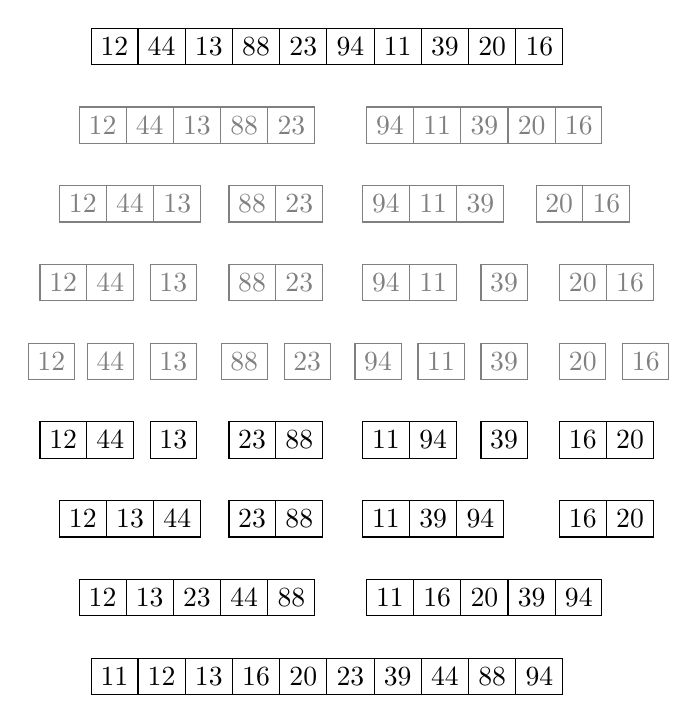
\begin{tikzpicture}[ level 1/.style={sibling distance=30mm}, level
  2/.style={sibling distance=30mm}, level 3/.style={sibling
    distance=20mm}]
  % Layer 0
  \node[array,rectangle split parts=10] at (-0.25,0)
  {12
    \nodepart{two}44
    \nodepart{three}13
    \nodepart{four}88
    \nodepart{five}23
    \nodepart{six}94
    \nodepart{seven}11
    \nodepart{eight}39
    \nodepart{nine}20
    \nodepart{ten}16 };

  % Layer 1
  \node[style=array, rectangle split parts=5,color=gray] at (-1.9,-1)
  {12
    \nodepart{two}44
    \nodepart{three}13
    \nodepart{four}88
    \nodepart{five}23
  };
  \node[array,rectangle split parts=5,color=gray] at (1.75,-1)
  {94
    \nodepart{two}11
    \nodepart{three}39
    \nodepart{four}20
    \nodepart{five}16
  };

  % Layer 2
  \node[array, rectangle split parts=3,color=gray] at (-2.75,-2)
  {12
    \nodepart{two}44
    \nodepart{three}13
  };
  \node[array, rectangle split parts=2,color=gray] at (-.9,-2)
  {88
    \nodepart{two}23
  };
  \node[array, rectangle split parts=3,color=gray] at (1.1,-2)
  {94
    \nodepart{two}11
    \nodepart{three}39
  };
  \node[array, rectangle split parts=2,color=gray] at (3,-2)
  {20
    \nodepart{two}16
  };

  
  % Layer 3
  \node[array, rectangle split parts=2,color=gray] at (-3.3,-3)
  {12
    \nodepart{two}44
  };
  \node[array, rectangle split parts=1,color=gray] at (-2.2,-3)
  {13};
  \node[array, rectangle split parts=2,color=gray] at (-.9,-3)
  {88
    \nodepart{two}23
  };
  \node[array, rectangle split parts=2,color=gray] at (0.8,-3)
  {94
    \nodepart{two}11
  };
  \node[array, rectangle split parts=1,color=gray] at (2,-3)
  {39};
  \node[array, rectangle split parts=2,color=gray] at (3.3,-3)
  {20
    \nodepart{two}16
  };
  
  
  % Layer 4
  \node[array, rectangle split parts=1,color=gray] at (-3.75,-4)
  {12
  };
  \node[array, rectangle split parts=1,color=gray] at (-3,-4)
  {44};
  \node[array, rectangle split parts=1,color=gray] at (-2.2,-4)
  {13};
  \node[array, rectangle split parts=1,color=gray] at (-1.3,-4)
  {88};
  \node[array, rectangle split parts=1,color=gray] at (-.5,-4)
  {23};

  \node[array, rectangle split parts=1,color=gray] at (.4,-4)
  {94
  };
  \node[array, rectangle split parts=1,color=gray] at (1.2,-4)
  {11};
  \node[array, rectangle split parts=1,color=gray] at (2,-4)
  {39};
  \node[array, rectangle split parts=1,color=gray] at (3,-4)
  {20};
  \node[array, rectangle split parts=1,color=gray] at (3.8,-4)
  {16};

  % Layer 5
  \node[array, rectangle split parts=2] at (-3.3,-5)
  {12
    \nodepart{two}44
  };
  \node[array, rectangle split parts=1] at (-2.2,-5)
  {13};
  \node[array, rectangle split parts=2] at (-.9,-5)
  {23
    \nodepart{two}88
  };

  \node[array, rectangle split parts=2] at (0.8,-5)
  {11
    \nodepart{two}94
  };
  \node[array, rectangle split parts=1] at (2,-5)
  {39};
  \node[array, rectangle split parts=2] at (3.3,-5)
  {16
    \nodepart{two}20
  };

  % Layer 6
  \node[array, rectangle split parts=3] at (-2.75,-6)
  {12
    \nodepart{two}13
    \nodepart{three}44
  };
  \node[array, rectangle split parts=2] at (-.9,-6)
  {23
    \nodepart{two}88
  };
  \node[array, rectangle split parts=3] at (1.1,-6)
  {11
    \nodepart{two}39
    \nodepart{three}94
  };
  \node[array, rectangle split parts=2] at (3.3,-6)
  {16
    \nodepart{two}20
  };

  % Layer 7
  \node[style=array, rectangle split parts=5] at (-1.9, -7)
  {12
    \nodepart{two}13
    \nodepart{three}23
    \nodepart{four}44
    \nodepart{five}88
  };
  \node[style=array, rectangle split parts=5] at (1.75, -7)
  {11
    \nodepart{two}16
    \nodepart{three}20
    \nodepart{four}39
    \nodepart{five}94
  };
  
  \node[array,rectangle split parts=10] at (-0.25,-8)
    {11
      \nodepart{two}12
      \nodepart{three}13
      \nodepart{four}16
      \nodepart{five}20
      \nodepart{six}23
      \nodepart{seven}39
      \nodepart{eight}44
      \nodepart{nine}88
      \nodepart{ten}94 };
\end{tikzpicture}
\caption{Problem 13: Merge Sort}
\label{p13ms}
\end{figure}

\question
\textbf{Insertion Sort}. For insertion sort, if the array is sorted or almost sorted, the algorithm will only do comparisons from first element to the last element($n$ times) and a small number of swaps(constant time). Hence, the time complexity for insertion sort is $\mathcal{O}(n)$ for best case(the array is sorted or almost sorted).

\question
When the pivots are always the minimum number or the maximum number of the sequence(or sub-sequence). In this case, either left or right part will be extremely long after parition. So, the recursion tree will be totally unbalanced with height $n$, which result in the final time complexity is $\mathcal{O}(n^2)$.

\question
\begin{enumerate}
  \item selection sort: \textbf{pros}: It's an in-place sorting algorithm. \textbf{cons}: In general cases, It takes more time to sort than merge sort and quick sort.
  \item insertion sort: \textbf{pros}: It's stable and it has the greatest performance when dealing with almost sorted list. \textbf{cons}:In general cases, It takes more time to sort than merge sort and quick sort.
  \item merge sort: \textbf{pros}: It's a stable sorting algorithm. Also, it's fast in general cases. \textbf{cons}: It takes extra spaces to store sub-array.
  \item quick sort: \textbf{pros}: It's the fastest algorithm compared with above three. \textbf{cons}: It's not stable and It will have bad performance in the worst case.
\end{enumerate}


\let\section=\defaultsection
\section*{Credits}
This assignment is written by \LaTeX with \href{https://github.com/jez/latex-homework-class}{template} under MIT License.

\end{document}
